\chapter{Writing your own Procedures and Functions}
\index{User defined Procedures and Functions}
This chapter will show you how you can eliminate the {\tt GOSUB}
instruction once and for all and not be reliant on line numbers
for your programs.

\section{User defined Procedures}
\index{User defined Procedures and Functions!Procedures}
Procedures (and functions) have a name, so just like variable names,
make them something that's easy to understand. We'll start by example
and write a procedure to print out a multiplication table:
\begin{verbatim}
  500 REM Procedure to print a multiplication table
  510 DEF PROC multiplication
  520 FOR num = 1 to 10 CYCLE
  530   PRINT num; " * "; table; " = "; num * table
  540 REPEAT
  550 ENDPROC
\end{verbatim}
We've given it a high line number to start with as procedures (and
functions) should be at the end of your program\footnote{This isn't
strictly necessary, but if the RTB system sees the {\tt DEF}\index{User
defined Procedures and Functions!DEF} keyword in normal program flow
then it will consider it an error and stop. You could put them all at
the top, then use a {\tt GOTO} instruction to jump over them, but some
may consider that inelegant!}.

Understanding the above: {\tt DEF PROC\index{User defined Procedures and
Functions!DEF PROC}} tells the system to define a
new procedure and call it {\tt multiplication}. The procedure
uses a global variable called {\tt table} to represent the 
table to be printed.

Demonstration of the above procedure, used to
print the 2,4,6 and 8 times tables:
\begin{verbatim}
  100 REM Print some tables
  110 FOR table = 2 TO 8 STEP 2 CYCLE
  230   PROC multiplication
  240 REPEAT
  250 END
\end{verbatim}
{\tt PROC}\index{User defined Procedures and
Functions!PROC} without the {\tt DEF} calls the procedure.

Like built-in procedures and functions, we can give our procedures
arguments. They can also have variables local to themselves.

Re-writing with an argument and local variable:
\begin{verbatim}
  500 REM Procedure to print a multiplication table
  510 DEF PROC multiplication (table)
  515 LOCAL num
  520 FOR num = 1 to 10 CYCLE
  530   PRINT num; " * "; table; " = "; num * table
  540 REPEAT
  550 ENDPROC
\end{verbatim}
and our calling program is now:
\begin{verbatim}
  100 REM Print some tables
  110 FOR table = 2 TO 8 STEP 2 CYCLE
  230   PROC multiplication (table)
  240 REPEAT
  250 END
\end{verbatim}

\section{User defined Functions}
\index{User defined Procedures and Functions!Functions}
Functions work in almost exactly the same was as procedures. We can
give them parameters and declare {\tt LOCAL} variables, however the
one difference is that a function can return a result, and you do this
by ending the function with the value to return after an equals symbol
{\tt =}\index{User defined Procedures and Functions!=} as this simple
example demonstrates:
\begin{verbatim}
  100 REM Function test - print squares
  110 FOR i = 1 TO 10 CYCLE
  130   x = FN square (i)
  140   PRINT i; " squared is"; x
  150 REPEAT
  160 END
  500 REM Function to return the square of a number
  510 DEF FN square (num)
  520 LOCAL result
  530 result = num * num
  540 = result
\end{verbatim}
You can use user-defined functions anywhere you might use a built-in
function, and you can define functions that return strings too -- just
make sure its name ends with a dollar sign.

This example reverses a string:
\begin{verbatim}
  500 REM Function to reverse a string
  510 DEF FN reverse$ (s$)
  520 LOCAL i
  530 LOCAL new$
  540 new$ = "" // Start with nothing
  550 FOR i = 1 to LEN (s$) CYCLE
  560   new$ = new$ + MID$ (s$, LEN (s$) - i, 1)
  570 REPEAT
  580 = new$
\end{verbatim}
  

\section{Recursion}
\index{Recursion}
Recursion is when a procedure or function calls itself.

Here is an example -- The factorial\index{Recursion!Factorial} function
is defined as the number multiplied by one less than itself multiplied
by one less than that and so on until you reach one.

e.g. 5 factorial is 5 * 4 * 3 * 2 * 1 (or 120)

A way of representing this is to say that 5 factorial
is 5 times 4 factorial.

We know that 4 factorial is 4 times 3 factorial, \dots

We also know that 1 factorial is 1 (and that we normally use the
exclamation mark to represent the factorial function)

So in general terms as can say that $N! = N * (N - 1)!$

If you're having problems thinking that one through, think of Russian
matryoshka dolls\index{Matryoshka dolls} -- A matryoshka doll is a
matryoshka doll with another matryoshka doll inside\dots

\noindent
Have a look at this function:
\begin{verbatim}
  500 DEF FN factorial (n)
  510 IF n = 1 THEN = n
  520 = n * FN factorial (n - 1)
\end{verbatim}

A an excercise, write a program to test this. How big a number can you
give it?\footnote{And did you just pick numbers ar random or use a {\tt
FOR} loop to count up?}

Now think about the string reversal function earlier. Can it be written
using recursion? If you think it can, then give it a go\footnote{If
stuck, then think of it this way: a reversed string is the
last character in a string followed by the rest of the string, reversed}.

But \meek before you get carried away with recursion, is it always the
best way? Who knows -- each case will be different. Think back to the
factorial example -- wouldn't it just have been easier to write it using
a {\tt FOR} loop? Give it a go and see what you think.

And if you want a recursive challenge, try this: You have a board with
three short wooden rods. On one rod is 5 different sized disks with a
hole in the middle to slide down the rod. Each disk is a different size
and the largest is at the bottom and the smallest at the top. See the
picture below.

Your task is to move them from one pole to another, but you must
never place a larger disk on top of a smaller one and you can only
move one disk at a time. This puzzle is called the {\sl Towers of
Hanoi}\index{Recursion!Towers of Hanoi} and is one of the old ``classic''
problems where a recursive solution works well.
\noindent
\begin{center}
{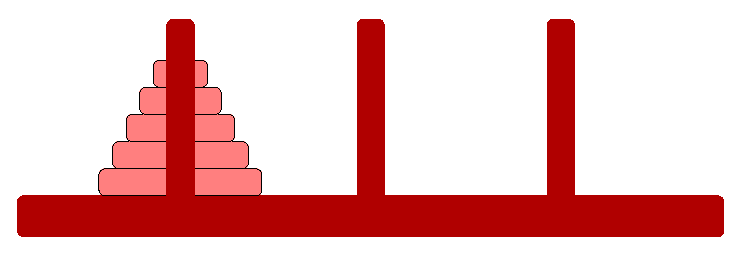
\includegraphics{hanoi.eps}}\\{\sl The Towers of Hanoi}
\end{center}

\section{Variable Scope}
\index{Variables!Scope}
We talk about the ``scope'' of a variable to mean what parts of your
program can see a variable (and change it!) We've seen that subroutines
can see (and change!) all variables we use in the main program, but what
about user defined procedures and functions?

The rules in RTB are somewhat simple, and whilst not identical, are
similar enough to most other progrmaming languages to give you a good
insight.

When a procedure or function is called, the arguments and {\tt LOCAL}
variables store a copy of any variables with the same name, making them
avalable for use inside that procedure or function. When the procedure
ends, then the stored values are copied back into the original variables.

So what happens if a procedure calls another procedure which doesn't
have local variables? Well, the values it sees are those of the last
procedure and not those in the main program. Essentially, RTB propogates
local variables into each new procedure. The easiest way to demonstrate is
by example:
\begin{verbatim}
  100 REM Variable Scope Test
  110 v1 = 123
  120 v2 = 456
  130 PROC test1 (v1)
  140 PRINT "v1 is: "; v1; " v2 is "; v2
  150 END
  300 REM test1
  310 DEF PROC test1 (num1)
  320 LOCAL v1
  330 v1 = 888
  340 PRINT "v1 is: "; v1; " v2 is "; v2; " num1 is: "; num1
  350 PROC test2
  360 ENDPROC
  500 //
  510 REM test2
  520 //
  530 DEF PROC test2
  340 PRINT "v1 is: "; v1; " v2 is "; v2; " num1 is: "; num1
\end{verbatim}
